\documentclass[ignorenonframetext,]{beamer}
\usetheme{Warsaw}
\usepackage{amssymb,amsmath}
\usepackage{ifxetex,ifluatex}
\usepackage{fixltx2e} % provides \textsubscript
\ifxetex
  \usepackage{fontspec,xltxtra,xunicode}
  \defaultfontfeatures{Mapping=tex-text,Scale=MatchLowercase}
\else
  \ifluatex
    \usepackage{fontspec}
    \defaultfontfeatures{Mapping=tex-text,Scale=MatchLowercase}
  \else
    \usepackage[utf8]{inputenc}
  \fi
\fi

\usepackage{minted}

% Comment these out if you don't want a slide with just the
% part/section/subsection/subsubsection title:
\AtBeginPart{
  \let\insertpartnumber\relax
  \let\partname\relax
  \frame{\partpage}
}
\AtBeginSection{
  \let\insertsectionnumber\relax
  \let\sectionname\relax
  \frame{\sectionpage}
}
\AtBeginSubsection{
  \let\insertsubsectionnumber\relax
  \let\subsectionname\relax
  \frame{\subsectionpage}
}

\setlength{\parindent}{0pt}
\setlength{\parskip}{6pt plus 2pt minus 1pt}
\setlength{\emergencystretch}{3em}  % prevent overfull lines
\setcounter{secnumdepth}{0}

\title{Introduction to Asynchronous Programming in Python}
\author{Antoine Pietri}
\date{2013-12-06}

\begin{document}
\frame{\titlepage}

\section{Introduction}

\begin{frame}[fragile]\frametitle{Synchronous I/O}

\begin{itemize}[<+->]
\itemsep1pt\parskip0pt\parsep0pt
\item
  In the vast majority of server applications, the limiting factor is
  I/O
\item
  An I/O request is blocking by default
\item
  All the CPU time is wasted waiting for the request to complete
\end{itemize}

\end{frame}

\begin{frame}\frametitle{Synchronous I/O diagram}

\begin{center}
 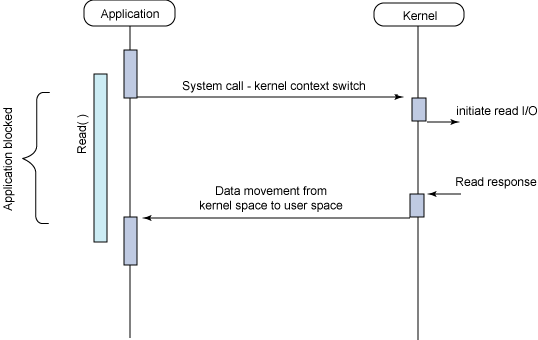
\includegraphics[height=6cm]{img/synchronous.png}
\end{center}

\end{frame}

\begin{frame}[fragile]\frametitle{Note on Synchronous I/O}

\begin{itemize}[<+->]
\itemsep1pt\parskip0pt\parsep0pt
\item
  There are some ways of making synchronous I/O non blocking
\item
  fcntl() with the O\_NONBLOCK flag allows non-blocking read/write
  requests
\item
  Synchronous non/blocking I/O is a perfectly valid way to make
  efficient I/O
\item
  But that's not the subject of this presentation anyway
\end{itemize}

\end{frame}

\begin{frame}[fragile]\frametitle{Asynchronous I/O}

\begin{itemize}[<+->]
\itemsep1pt\parskip0pt\parsep0pt
\item
  We need a way to keep the CPU busy
\item
  We can't afford to waste all the CPU time waiting for some I/O
  requests to complete
\item
  We could use asynchronous blocking I/O (select(2), poll(2), epoll(7),
  kqueue(7)), but that's tedious
\item
  In some high-level languages (Python!) we can use Coroutines to do
  that easily
\end{itemize}

\end{frame}

\begin{frame}[fragile]\frametitle{Synchronous I/O diagram}

\begin{center}
 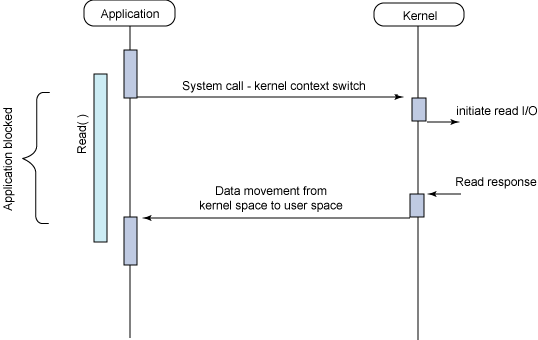
\includegraphics[height=6cm]{img/synchronous.png}
\end{center}

\end{frame}

\section{Generators and coroutines}

\begin{frame}[fragile]\frametitle{Disclaimer}

\begin{itemize}[<+->]
\itemsep1pt\parskip0pt\parsep0pt
\item
  Python \textgreater{}= 3.3
\item
  PEP 380
\item
  yield from
\item
  Returning from a function
\end{itemize}

\end{frame}

\begin{frame}[fragile]\frametitle{Generators}

\footnotesize{
\begin{minted}{python}

    def make_generator():
        yield 0
        yield 1

    g = make_generator()

    print(g)
    # <generator object make_generator at 0x7fe98ec66690>

    print(next(g))
    # 0
    print(next(g))
    # 1
    print(next(g))
    # Exception: StopIteration

\end{minted}
}

\end{frame}

\begin{frame}[fragile]\frametitle{Generators}

\footnotesize{
\begin{minted}{python}
    def make_generator():
        print('Start')
        yield 0
        print('Next')
        yield 1
        print('End')

    g = make_generator()

    print(next(g))
    # Start
    # 0
    print(next(g))
    # Next
    # 1
    print(next(g))
    # End
    # Exception: StopIteration
\end{minted}
}

\end{frame}

\begin{frame}[fragile]\frametitle{Generators}

Easy way to have ``laziness'' in Python:

\footnotesize{
\begin{minted}{python}
    def get_pages():
        for i in range(10):
            yield requests.get(
                'http://example.com/page/{}'.format(i)).text

    def main():
        for p in get_pages():
            print(p)
\end{minted}
}

\end{frame}

\begin{frame}[fragile]\frametitle{Coroutines}

\begin{itemize}[<+->]
\itemsep1pt\parskip0pt\parsep0pt
\item
  A coroutine is a routine that can be suspended and resumed
\item
  Cohabits with the routines, with a different context stack
\item
  Very handful for Asynchronous I/O
\item
  Added in Python in PEP 342 (``Coroutines via enhanced generators'')
\end{itemize}

\end{frame}

\begin{frame}[fragile]\frametitle{Coroutines}

\begin{center}
 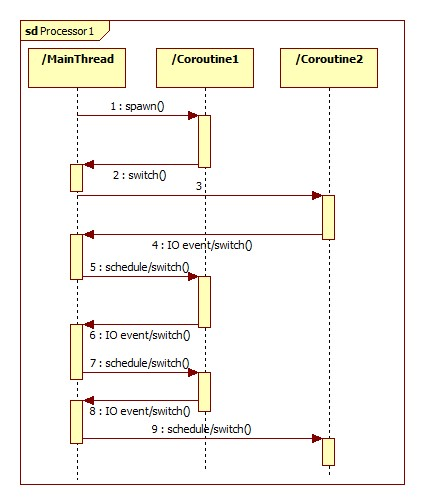
\includegraphics[height=6cm]{img/coroutine_diagram}
\end{center}

\end{frame}

\begin{frame}[fragile]\frametitle{Coroutines}

Let's take our previous example:

\begin{minted}{python}
    def main():
        for p in get_pages():
            print(p)
\end{minted}

\end{frame}

\begin{frame}[fragile]\frametitle{Coroutines}

It can be rewritten like this:

\begin{minted}{python}
    def main():
        generator = get_pages()
        while True:
            try:
                print(next(generator))
            except StopIteration:
                break
\end{minted}

\begin{itemize}[<+->]
\itemsep1pt\parskip0pt\parsep0pt
\item
  We can see the explicit call to next(), which \emph{resumes} the
  coroutine.
\item
  But maybe we could send something, when resuming this coroutine?
\end{itemize}

\end{frame}

\begin{frame}[fragile]\frametitle{Coroutines}

This is equivalent to:

\begin{minted}{python}

    def main():
        generator = get_pages()
        while True:
            try:
                print(generator.send(None))
            except StopIteration:
                break

\end{minted}

\begin{itemize}[<+->]
\itemsep1pt\parskip0pt\parsep0pt
\item
  A generator is a coroutine
\item
  A call to next() is a call to .send() with the None value.
\end{itemize}

\end{frame}

\begin{frame}[fragile]\frametitle{Coroutines}

\begin{itemize}[<+->]
\itemsep1pt\parskip0pt\parsep0pt
\item
  We can communicate with our coroutine by sending values!
\item
  Every generator can be resumed with their method send(value)
\end{itemize}

\end{frame}

\begin{frame}[fragile]\frametitle{Coroutines}

\footnotesize{
\begin{minted}{python}
    def make_coroutine():
        val = yield 1
        print('coroutine got {}'.format(val))
        val = yield 2
        print('coroutine got {}'.format(val))

    def main():
        coroutine = make_coroutine()
        i = coroutine.send(None) # starts coroutine
        while True:
            try:
                print('main() retrieved {}'.format(i))
                print(coroutine.send(i * 2))
            except StopIteration:
                break
\end{minted}
}

\end{frame}

\begin{frame}[fragile]\frametitle{yield from}

\begin{minted}{python}
    yield from coroutine
\end{minted}

\begin{itemize}[<+->]
\itemsep1pt\parskip0pt\parsep0pt
\item
  Added in Python 3.3 (PEP 380)
\item
  Acts as a ``pipe'' between coroutines
\end{itemize}

\end{frame}

\begin{frame}[fragile]\frametitle{yield from}

\tiny{
\begin{minted}{python}
    def coroutine1():
        a = 0
        while True:
            a = yield a
            a += 10

    def coroutine2():
        yield 42
        yield 1337
        yield from coroutine1()

    def main():
        a = 3
        c = coroutine2()
        while True:
            try:
                a = c.send(a)
                print(a)
            except StopIteration:
                break
    # 42, 1337, 3, 13, 23...
\end{minted}
}

\end{frame}

\section{Coroutines for Async I/O}

\begin{frame}[fragile]\frametitle{Explanation}

\begin{itemize}[<+->]
\itemsep1pt\parskip0pt\parsep0pt
\item
  So, how coroutines and Async I/O are actually related?
\item
  The other common way of making Asynchronous I/O is using callback, but
  that's pretty verbose
\item
  In each case, you need to run an event-loop somewhere.
\end{itemize}

\end{frame}

\begin{frame}[fragile]\frametitle{Callbacks}

\tiny{
\begin{minted}{python}
    content = b''

    def read_async(fd):
        read(fd, callback=on_read_received)
        print('Not blocking!')

    def on_read_received(fd, data):
        print('Received data on fd {}'.format(fd))
        content += data

\end{minted}
}

\normalsize{
\begin{itemize}[<+->]
\itemsep1pt\parskip0pt\parsep0pt
\item
  The framework provides base functions (read/write/\ldots{}) that uses
  internally I/O operations in their eventloop (using kqueue,
  epoll or select)
\item
  This is extremely verbose, due to the fact we're constantly changing
  routines
\item
  At least we achieved our goal! We can launch ``parallels'' reads,
  instead of waiting at each blocking read.
\end{itemize}
}

\end{frame}

\begin{frame}[fragile]\frametitle{Callbacks}

\begin{minted}{python}
    read_async(10) # (takes a fd)
    read_async(1)
    read_async(3)
    print('You see, not blocking !')

    # You see, not blocking !
    # Received data on fd 1
    # Received data on fd 10
    # Received data on fd 3
\end{minted}

\end{frame}

\begin{frame}[fragile]\frametitle{Futures}

\begin{itemize}[<+->]
\itemsep1pt\parskip0pt\parsep0pt
\item
  What if we used \textbf{yield points} instead of callbacks?
\item
  Instead of taking a callback parameter, functions of the framework
  returns \textbf{futures}.
\item
  When you yield a future, you ``give back the hand'' to your event loop
\item
  The event loop resumes your coroutine when the result is ready
\end{itemize}

\end{frame}

\begin{frame}[fragile]\frametitle{Futures}

\begin{minted}{python}
    content = b''
    def read_async(fd):
        future = read(fd, callback=on_read_received)
        print('Not blocking!')

        data = yield future # "Yield point"
        content += data
\end{minted}

\end{frame}

\begin{frame}[fragile]\frametitle{Futures}

\begin{itemize}[<+->]
\itemsep1pt\parskip0pt\parsep0pt
\item
  The I/O is no longer blocking, your coroutine is just ``resumed'' when
  the data is ready
\item
  It means you can do effective I/O, without wasting your CPU time
  waiting for blocking I/O
\end{itemize}

\end{frame}

\begin{frame}[fragile]\frametitle{Futures}

In the case of a web server:

\begin{minted}{python}
    handle_GET_request(sloooow_client)
    handle_GET_request(fast_client)
    handle_GET_request(not_very_fast_client)
    handle_GET_request(fast_client)

    # fast_client request handled!
    # fast_client request handled!
    # not_very_fast_client request handled!
    # sloooow_client request handled!
\end{minted}

\end{frame}

\section{Frameworks}

\begin{frame}[fragile]\frametitle{Gevent}

\begin{itemize}[<+->]
\itemsep1pt\parskip0pt\parsep0pt
\item
  Certainly the most known/used event library in Python 2
\item
  No official support for Python 3, although some ports exist
\item
  Weird implementation (x86 CPython specific bytecode)
\item
  Monkey-patching: not nicely behaving with the standard library
\item
  Everything is async by default: no explicit yield-points
\end{itemize}

\end{frame}

\begin{frame}[fragile]\frametitle{Twisted}

\begin{itemize}[<+->]
\itemsep1pt\parskip0pt\parsep0pt
\item
  Good alternative, using ``Deferred'' for futures
\item
  Similar mecanism
\item
  A bit bloated
\item
  Very hard to understand at first
\end{itemize}

\end{frame}

\begin{frame}[fragile]\frametitle{Tornado}

\begin{itemize}[<+->]
\itemsep1pt\parskip0pt\parsep0pt
\item
  Web-oriented framework
\item
  Very efficient
\item
  Long-polling, websockets, HTTP streaming\ldots{}
\item
  Relies heavily on callbacks by design
\item
  Light coroutine ``syntastic sugar'' have been around for a while
\end{itemize}

\end{frame}

\begin{frame}[fragile]\frametitle{Toro}

\begin{itemize}[<+->]
\itemsep1pt\parskip0pt\parsep0pt
\item
  A library that provides synchronisation primitives for Tornado
  coroutines
\item
  A lot of gevent ideas ported to Tornado
\item
  Toro.Event(), Toro.Queue(), \ldots{}
\end{itemize}

\end{frame}

\begin{frame}[fragile]\frametitle{Tulip (asyncio)}

\begin{itemize}[<+->]
\itemsep1pt\parskip0pt\parsep0pt
\item
  PEP 3156: Asynchronous IO Support Rebooted
\item
  Goal: standardize the event-loop in Python to allow interoperability
  between frameworks
\item
  Relies a lot on \textbf{yield from} to communicate with the
  event-loop.
\end{itemize}

\begin{minted}{python}
    @tulip.coroutine
    def download(url):
        response = yield from http.request('GET', url)
        data = yield from response.read()
\end{minted}

\end{frame}

\begin{frame}\frametitle{Questions?}

    antoine.pietri1@gmail.com

    \#epita @ irc.rezosup.org

    Slides available soon on http://gconfs.fr/confs

\end{frame}

\end{document}
